\documentclass[acmsmall,screen, nonacm]{acmart}
\usepackage{graphicx}
\AtBeginDocument{%
  \providecommand\BibTeX{{%
    Bib\TeX}}}

\begin{document}

\title{COSC 520 Assignment 2: Advanced Data Structures}

\author{Rishav Banerjee}
\email{rishavb@student.ubc.ca}
\affiliation{%
	\institution{University of British Columbia}
	\country{Canada}
}

\renewcommand{\shortauthors}{Banerjee}

\begin{abstract}
	This document details the process of profiling 3 advanced data structures for fuzzy searching: BK-Trees, VP-Trees and Tries.
	The open source code can be found at \url{https://github.com/ThatAmuzak/COSC-520-Assignments} under the \texttt{Assignment 2} subdirectory.
\end{abstract}

\received{\today}

\maketitle

\section{Introduction}

Fuzzy matching is the task of finding strings in a collection that are ``close'' to a query string, where closeness is measured by an edit-distance function.
Edit distance metrics quantify how many primitive operations (typically insertions, deletions, and substitutions) are required to transform one string into another.
A common and widely used edit distance is the \emph{Levenshtein distance}~\cite{wikipediaLevenshteinDistance}, which counts the minimum number of single-character insertions, deletions, and substitutions needed to convert one string to another.
The Levenshtein distance is commonly computed using dynamic programming (Wagner--Fischer style algorithms) and is the principal distance metric used in this project.

Other edit-distance variants also exist (for example, Damerau--Levenshtein, which also counts adjacent transpositions). A number of algorithmic approaches exist to compute or approximate these distances; this document focuses on using an exact Levenshtein-distance computation (Wagner--Fischer DP) as the underlying metric, and on profiling three different data structures (plus a linear array baseline) for supporting efficient fuzzy search over large dictionaries.

\section{Personal Relevance (HCI context)}
Fuzzy matching is closely related to human text entry: when users type on keyboards (physical or soft), errors occur (misspellings, omissions, transpositions), and fuzzy matching enables tolerant lookup and correction. Applications include spell checkers, autocomplete / suggestion systems, fuzzy database lookups (e.g., name matching), automated assessment of free-text responses, and many text-entry assistive techniques studied in HCI. In text-entry research, fuzzy matching underpins research into error-tolerant keyboards and predictive text algorithms, where tolerant lookup improves perceived system responsiveness and reduces user effort.

\section{Data Structures}
We compare three structured indexes and a simple array baseline. For each structure we describe origin, core idea, and how fuzzy search is performed with Levenshtein distance.

\subsection{BK-Trees}
\paragraph{Overview and Origin.}
A BK-tree (Burkhard--Keller tree)~\cite{wikipediaBKtreeWikipedia} is a metric tree specialized to discrete metric spaces. It was first proposed by Burkhard and Keller in the early 1970s. The tree stores terms at nodes; each edge from a node to a child is labeled by the metric distance between the node's term and the child's term. The BK-tree exploits the triangle inequality to prune subtrees that cannot contain points within a requested distance of the query.

\paragraph{Structure and Search.}
To insert a word into a BK-tree: if the tree is empty the word becomes the root. Otherwise, compute the distance $d$ between the word and the current node's term; follow the child edge labeled $d$ if present, or create it if absent, and continue recursively. For query-time fuzzy search (given a query $q$ and threshold $t$): start at the root, compute $d=\mathrm{dist}(q, node\_term)$ and if $d\le t$ record the node term as a match. Then recursively visit children whose edge labels $e$ satisfy $e\in [d - t,\; d + t]$; by triangle inequality any child outside that window cannot contain a point within distance $t$ of $q$.

\paragraph{Example.}
A small example: insert words \texttt{"book"}, \texttt{"back"}, \texttt{"bat"}, \texttt{"cook"} using Levenshtein distance; searching for \texttt{"bok"} with $t=1$ will examine nodes whose label edges are within the $[d-t,d+t]$ window and return close spellings efficiently.

\subsection{VP-Trees}
\paragraph{Overview and Origin.}
A vantage-point tree (VP-tree)~\cite{wikipediaVantagepointTree} is a metric-partitioning data structure that recursively partitions points around a chosen \emph{vantage point}. The VP-tree construction and analysis were popularized in work by Yianilos (and earlier by Uhlmann and others) for nearest-neighbor search in general metric spaces.

\paragraph{Structure and Search.}
To build a VP-tree: choose a vantage point (a point from the set), compute distances from that vantage point to all other points, pick a median distance $\mu$ and partition the set into an \emph{inner} subset (distance $\le\mu$) and an \emph{outer} subset (distance $>\mu$). Store the vantage point and the radius $\mu$ at the node and recurse on inner and outer subsets to form children. At query time, compute distance $d=\mathrm{dist}(q, vp)$; any subtree whose radius interval intersects the query window $[d- t, d+ t]$ may contain matches and must be visited. The VP-tree is flexible and often yields good pruning behavior in high-dimensional or non-euclidean metric spaces when the distribution of distances is favorable.

\subsection{Tries (Prefix Trees)}
\paragraph{Overview and Origin.}
A \emph{trie} (or prefix tree)~\cite{wikipediaTrieWikipedia} is a tree-like dictionary structure that stores keys by their prefixes; the term ``trie'' (from \emph{retrieval}) is commonly associated with Fredkin's discussion of trie memory in the 1960s. Tries are particularly useful when many words share common prefixes: common prefixes are only stored once, which reduces memory overhead and allows very fast exact-prefix search.

\paragraph{Approximate Search with Levenshtein DP Rows.}
We use an algorithm that traverses the trie while maintaining a Levenshtein DP row at each node. The technique (popularized in many implementations and tutorials) operates as follows: for each trie node corresponding to a prefix $p$, keep the current DP row that represents the distances between the query and the prefix $p$. When descending to a child representing adding character $c$, compute the next DP row from the parent's DP row using the standard Levenshtein recurrence for the new character. A node is a match if it is terminal and the DP row's last cell (distance between query and full word) is $\le\texttt{maxDist}$. Additionally, if the minimum value in the DP row is greater than \texttt{maxDist}, the entire subtree can be pruned because no extension of this prefix can produce a close enough word.

This traversal-with-DP approach achieves substantial pruning when many words share prefixes and when \texttt{maxDist} is small.

\subsection{Summary}

Table \ref{tab:complexities_concise} summarizes all the time and space complexities between the different data structures compared.

\begin{table}[ht]
	\centering
	\small
	\begin{tabular}{|l|c|c|c|}
		\hline
		\textbf{Structure} & \textbf{Build}             & \textbf{Fuzzy search}               & \textbf{Space} \\
		\hline
		Array (baseline)   & $O(n)$                     & $O(n\cdot L\cdot Q)$                & $O(n\cdot L)$  \\
		\hline
		BK-tree            & $O(n\log n\cdot L\cdot Q)$ & $O(\log n\cdot L\cdot Q)$ (typ.)    & $O(n\cdot L)$  \\
		\hline
		VP-tree            & $O(n\log n\cdot L\cdot Q)$ & $O(\log n\cdot L\cdot Q)$ (typ.)    & $O(n\cdot L)$  \\
		\hline
		Trie               & $O(n\cdot L)$              & $O(V\cdot Q)$\ ($V=$ nodes visited) & $O(n\cdot L)$  \\
		\hline
	\end{tabular}
	\caption{Complexities: $n$ = number of words, $L$ = avg word length, $Q$ = query length, $V$ = trie nodes visited (depends on pruning).}
	\label{tab:complexities_concise}
\end{table}

\section{Implementation}

The implementation is organized as a single module that provides a clear Levenshtein distance function and three index types with small, stable build and search interfaces. Public routines are annotated with type hints and runtime checks to help catch incorrect usage early.

The Levenshtein distance routine is implemented as an exact dynamic programming algorithm that returns the integer edit distance between two strings. The implementation is compact and designed for efficiency in typical cases by minimizing memory allocations and using a rolling-row optimization where appropriate.

Each index type wraps that distance function and exposes two primary capabilities: a build operation that consumes a collection of words and constructs the internal representation, and a search operation that returns the nearest matches to a query string up to a requested count. The three indexed approaches differ in how they organize words and what pruning they can apply at query time. There is also a simple array baseline that performs an unindexed linear scan computing distances to every candidate and selecting the closest matches.

The BK-tree stores words at nodes with edges labeled by inter-term distances; this allows visiting only those child subtrees whose edge labels could contain matches within a chosen threshold. The VP-tree partitions words around vantage points and a median radius so that queries only search subtrees whose radius intervals intersect the query window. The trie stores words by prefixes and performs approximate search by maintaining the current Levenshtein DP row while traversing; terminal nodes whose DP last cell is within the allowed maximum are returned and branches are pruned when the DP row's minimum exceeds the allowed distance.

The code base includes a unit test suite exercising the distance function and representative build/find scenarios for each index. At the time this document was created all unit tests for the fuzzy matching implementations passed.

\section{Methodology (Profiling Process)}

All tests were conducted on a Windows Machine with Python 3.12.4.
The machine contains the following hardware: 12th Gen Intel(R) Core(TM) i5-12600K and 32 GB of DDR4 RAM.

The profiling methodology was designed to measure two distinct costs for each approach: the time required to construct the index for a given sample of words, and the time required to perform approximate lookups on that freshly built index. Results were gathered across a range of dataset sizes and across multiple repetitions to produce reliable summary statistics.

For each data structure and dataset size, a random query string of fixed length was generated to emulate typical misspellings. A configurable warmup phase exercised both build and search operations to reduce one-off effects such as interpreter warm-up or cold caches; warmup runs were not included in the recorded measurements.

Measurements used repeated trials. Each trial began by ensuring the runtime was in a clean state so that no previously built structure could influence the result. The build operation was then timed while constructing the index from the current sample of words. Immediately after build completion, the search operation was timed by issuing the approximate lookup for the prepared query. After each trial any produced state was cleared to guarantee that subsequent trials started from the same baseline.

Raw timing samples for both build and find tasks were collected across repetitions. After all repetitions for a cell completed, the harness computed simple summary statistics (minimum, mean, maximum, and standard deviation) to quantify central tendency and variability. Each measurement cell was recorded with identifying metadata (the data structure, the task name, and the dataset size) together with the complete list of per-trial times so that downstream analysis can compute other aggregations, produce plots, or perform statistical tests.

The unindexed array baseline was measured within the same framework. Its build cost is effectively the cost of selecting the subset of the dataset for the measurement, and its find cost is the cost of a linear scan that computes Levenshtein distance to every candidate and selects the smallest-distance items. Comparing this baseline to the indexed approaches highlights the trade-off between the indexing overhead and the query-time savings achieved by each structure.

The methodology emphasizes repeatability, noise mitigation through warmups and multiple repetitions, and preservation of raw timing data to support flexible post hoc analysis.

Note that only 1 million elements were tested with at most, as the profiling process was taking excessively long beyond that point.

\section{Results}

We present two main findings, the build times for the respective data structures, and the subsequent search times for the datastructures.

\subsection{Build Times}

\begin{figure}[H]
	\centering
	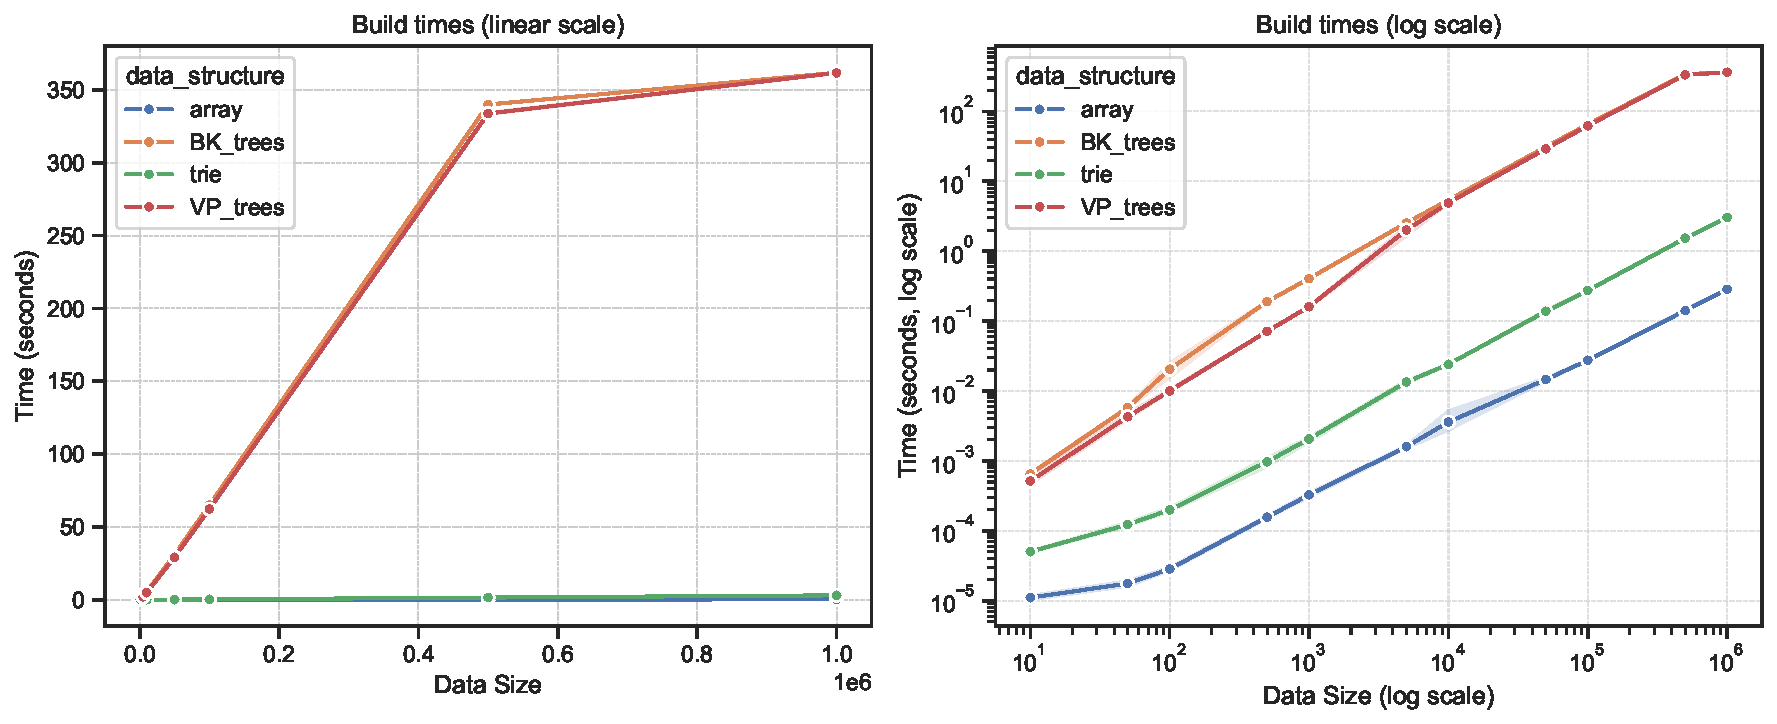
\includegraphics[width=1\textwidth]{build_times.pdf}
	\caption{Build time results showcasing the performance of the different functions, with 95\% confidence intervals in the shaded area. The left side graph shows without log scale and the right side with log scale. The color indicates the data structure utilized}
	\Description{Build time results showcasing the performance of the different functions, with 95\% confidence intervals in the shaded area. The left side graph shows without log scale and the right side with log scale. The color indicates the data structure utilized}
	\label{fig:pdfimage1}
\end{figure}

Key takeaways are as follows:
\begin{itemize}
	\item Build time increases roughly linearly with data size on a linear scale.
	\item Arrays exhibit the lowest build times across all data sizes.
	\item BK-trees and VP-trees show higher build times compared to arrays and tries.
	\item Trie structures perform moderately—faster than BK-trees and VP-trees but slower than arrays.
	\item VP-trees scale poorly with large datasets, showing the steepest increase in time.
\end{itemize}

\subsection{Search Times}

\begin{figure}[H]
	\centering
	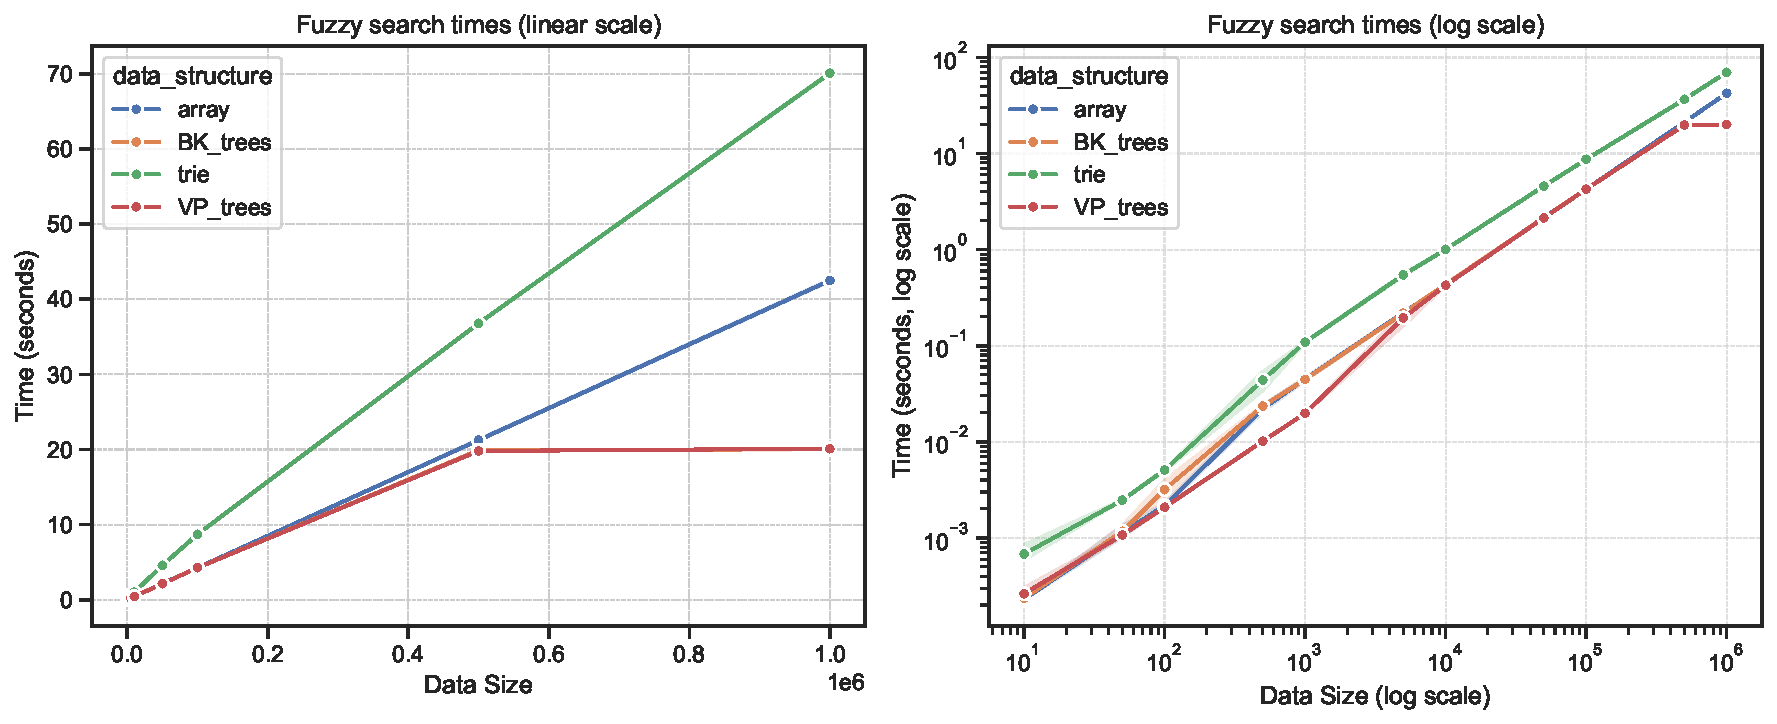
\includegraphics[width=1\textwidth]{search_times.pdf}
	\caption{Search time results showcasing the performance of the different functions, with 95\% confidence intervals in the shaded area. The left side graph shows without log scale and the right side with log scale. The color indicates the data structure utilized}
	\Description{Build time results showcasing the performance of the different functions, with 95\% confidence intervals in the shaded area. The left side graph shows without log scale and the right side with log scale. The color indicates the data structure utilized}
	\label{fig:pdfimage2}
\end{figure}

Key takaways are as follows:
\begin{itemize}
	\item Fuzzy search time increases with data size for all data structures.
	\item BK-trees moderately achieve the fastest search times, especially for larger datasets.
	\item VP-trees perform similarly to BK-trees and remain efficient at scale.
	\item Basic arrays remain competitive till we reach 1 million elements, showing for smaller datasets, they are both simple to implement and viable for fuzzy searching.
	\item Trie are significantly slower, showing the poorest scalability.
\end{itemize}

\section{Conclusion}
Thus we conclude this comparision between different advanced data structures for fuzzy searching. The open source code can be found at \url{https://github.com/ThatAmuzak/COSC-520-Assignments} under the \texttt{Assignment 2} subdirectory.

\section{AI Usage Declaration}
AI was used to assist with documentation of the program, and verify implemementations. All AI outputs were cross-validated.

\bibliographystyle{ACM-Reference-Format}
\bibliography{refs.bib}

\end{document}
\endinput
